\chapter[MonteCarlo samples production]{MonteCarlo production of Minimal DM model samples for the \mph analysis}
\label{chapt:mc}

\lettrine{T}{}his chapter describes all the steps made to generate, simulate and reconstruct MonteCarlo (MC) events in the context of the Minimal DM model for the \mph analysis .

%In the \mph analysis, which is a ``cut\&count'' analysis (refer to Chapt. \ref{chapt:mph}), we are looking for a single high energy photon and large missing transverse momentum (\met) signature, whose definition will be given in \Sect{\ref{sec:recoreal}}. Therefore it is characterized by a relative clean final state thanks also to a small set of SM processes that produces the same outcome. The Minimal DM model predicts several ways in which DM can be produced and revealed within a \mph analysis. Three examples of Feynman diagram are given in \Fig{\ref{fig:feynman}}. Notice that a photon can also be radiated from the final state which is a peculiarity with respect to other DM simplified models adopted at LHC.

The simulation of the physics processes in the detector is a fundamental ingredient in the analysis to assess the discovery potential for a new signal but also as input to the real data scrutiny.
%In order to study the detector response for a wide range of physics processes and scenarios, 
A detailed simulation  of the physics process and of the detector response is pursued providing an output format which is identical to that of the true detector. 

The simulation process of events comes across several steps. The first one is the event generation in which the products of \pp collision are simulated. The event generation starts with the creation of the list of particles (electrons, photons, partons\dots) from the hard scattering. The partons radiation is modeled through \emph{parton shower}, finally hadronization and underlying events are also used to complete the event. This step consists in the Truth-level simulation, producing an EVNT file, and a summary file (a TRUTH file) can be built from this events at particle level.

The second step consists in the simulation of how particles interact with the detector which is followed by the digitization of the events. The simulation program is integrated into the ATLAS software framework, Athena, and uses the \geant \cite{geant4} simulation toolkit. Detailed description of the ATLAS Simulation Infrastructure is given in~\cite{simulation}.

Afterwards the simulated event can be passed to the reconstruction software in the same way as actual recorded data. Then all the events reconstructed are filtered by a derivation code which selects only the  relevant events for a specific analysis. Finally the ``derivated'' events are collected in a compact and practical ROOT file, i.e a NTUPLE, ready to be processed by the analysis.

For this analysis the software chain described above, and shown in \Fig{\ref{fig:chain}}, was run in batch mode on the Milano Tier3 computing facility via HTCondor$^{\textup{TM}}$.


\begin{figure}[t]
\centering
{\fontfamily{pag}\selectfont  
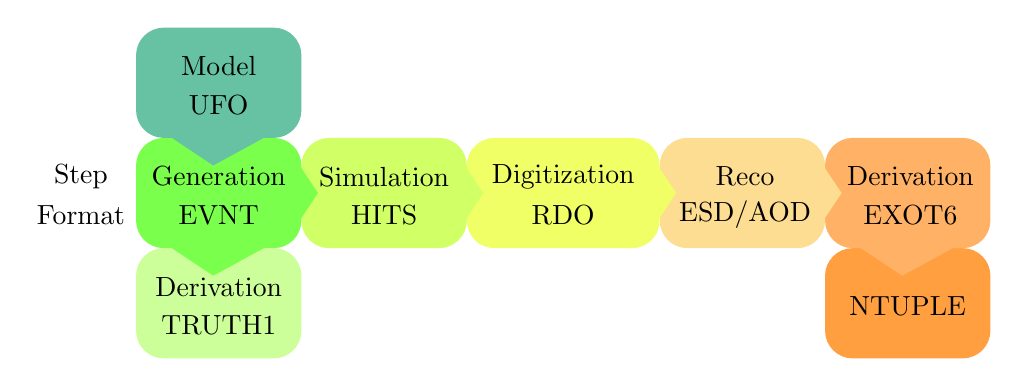
\begin{tikzpicture}[scale=0.7]

	\node[] at (-1,1.3){Step};
 	\node[] at (-1,0.6){Format};
 	
 	\draw[draw=none,fill=orange!75!, rounded corners=10pt] (12.5,0) rectangle +(3,-2);
 	\node[] at (1.5+12.5,-2+0.6+.35){NTUPLE};
 	
	\draw[draw=none,fill=orange!60!, rounded corners=10pt] (12.5,0) rectangle +(3,2);
 	\draw[draw=none,fill=orange!60!] (13,0.1)--(1.4+12.5,-0.5)--(2.5+12.5,0.1) -- cycle;
 	\node[] at (7.75+6.3,1.3){Derivation};
 	\node[] at (7.75+6.3,0.6){EXOT6};
	
	\draw[draw=none,fill=yellow!40!orange!40,rounded corners=10pt] (9.5,0) rectangle +(3,2);
 	\draw[draw=none,fill=yellow!40!orange!40] (12.4,0.4)--(12.8,1)--(12.4,1.6) -- cycle;
 	\node[] at (7.75+3.3,1.3){Reco};
 	\node[] at (7.75+3.3,0.6){ESD/AOD};
	
	\draw[draw=none,fill=green!10!yellow!60,rounded corners=10pt] (6,0) rectangle +(3.5,2);
 	\draw[draw=none,fill=green!10!yellow!60] (9.4,0.4)--(9.8,1)--(9.4,1.6) -- cycle;
 	\node[] at (7.75,1.3){Digitization};
 	\node[] at (7.75,0.6){RDO};
	
	\draw[draw=none,fill=green!30!yellow!60,rounded corners=10pt] (3,0) rectangle +(3,2);
 	\draw[draw=none,fill=green!30!yellow!60] (5.9,0.4)--(6.3,1)--(5.9,1.6) -- cycle;
 	\node[] at (4.5,1.3){Simulation};
 	\node[] at (4.5,0.6){HITS};
 	
 	\draw[draw=none,fill=green!75!yellow!70,rounded corners=10pt] (0,0) rectangle +(3,2);
	\draw[draw=none,fill=green!50!yellow!40,rounded corners=10pt] (0,0) rectangle +(3,-2);
 	\draw[draw=none,fill=green!75!yellow!70] (2.9,0.4)--(3.3,1)--(2.9,1.6) -- cycle;
 	\draw[draw=none,fill=green!75!yellow!70] (.5,0.1)--(1.4,-0.5)--(2.5,0.1) -- cycle;
 	
 	\node[] at (1.5,1.3){Generation};
 	\node[] at (1.5,0.6){EVNT};
 	\node[] at (1.5,-2+1.3){Derivation};
 	\node[] at (1.5,-2+0.6){TRUTH1};
 	
 	\draw[draw=none,fill=green!60!blue!60,rounded corners=10pt] (0,2) rectangle +(3,2);
 	\draw[draw=none,fill=green!60!blue!60] (.5,2.1)--(1.4,1.5)--(2.5,2.1) -- cycle;
 	\node[] at (1.5,3.3){Model};
 	\node[] at (1.5,2.6){UFO};
 	
 	%\node[] at (10.5,1.3){Reconstruction};
 	%\node[] at (10.5,0.6){ESD/AOD};

	%\node[ single arrow , draw, single arrow head extend=.7cm, gray!50, black] at (3.3,0.8) {    };
\end{tikzpicture}
}
\caption{The ATLAS simulation chain. The theoretical model is implemented in a UFO file and given as input to the generation program. Truth level analysis can be pursued, or the EVNT file can be used in a detector simulation whose outcome will be digitized in a RawData Object file and reconstructed in Event Summary Data (ESD) and Analysis Object Data (AOD). A derivation framework runs over the AOD to get the relevant events for a specific analysis. The Derivated Analysis Object Data (DAOD), which in our case is an EXOT6 file, can be made readable by RooT in a NTUPLE form.}
\label{fig:chain}
\end{figure}


\section{Generation}
 \begin{figure}[tp]
 \centering
 \begin{tikzpicture}
 [scale=0.5,decoration={
markings,% switch on markings
mark=% actually add a mark
at position .5  with {\arrow{>}}}]
 \draw[thick, postaction={decorate}] (-4,2) node at(-3,1)[above=2pt] {  $q$} -- (-2,0) ;
 \draw[thick, postaction={decorate}] (-2,0) -- (-4,-2) node at(-3,-1) [below=2pt] {  $\bar{q}$} ;
 \draw[thick,decorate,decoration={snake,amplitude=1.5mm,segment length=3.5mm}] (-2,0)--(1,0) node  at (-0.25,0) [below=3pt]{  $\gamma$,$\Zboson$};
 \draw[thick, postaction={decorate}] (1,0) -- (3,1) node at (2,0.5) [above]  {  $\chi^{\pm}$} ;
 \draw[thick, postaction={decorate}] (3,-1) --(1,0) node at (2,-0.5) [below=2pt]  {  $\chi^{\mp}$} ;
\draw[thick](3,1)--(3.4,2) node[above] {  $\pi^{\pm}$};
\draw[thick,postaction={decorate}](3,1)--(4.3,1.5) node[right=5pt,below] at (3.5,1.24) {  $\chi_0$};
\draw[thick](3,-1)--(3.4,-2) node[below] {  $\pimp$};
\draw[thick,postaction={decorate}](4.3,-1.5)--(3,-1) node[right=5pt,above] at (3.5,-1.24) {  $\chi_0$};
\draw[thick,decorate,decoration={snake,amplitude=1.5mm,segment length=8mm}] (-2.65,0.68)--(1,2) node at (-1,1.5) [above]{  $\gamma$};


 \draw[thick, postaction={decorate}] (-4+10,2) node at(-3+10,1)[above=2pt] {  $q$} -- (-2+10,0) ;
 \draw[thick, postaction={decorate}] (-2+10,0) -- (-4+10,-2) node at(-3+10,-1) [below=2pt] {  ${q'}$} ;
 \draw[thick,decorate,decoration={snake,amplitude=1.5mm,segment length=3.5mm}] (-2+10,0)--(1+10,0) node  at (-0.5+10,0) [below=3pt]{  $W^{\pm}$};
 \draw[thick, postaction={decorate}] (1+10,0) -- (3+10,1) node at (2+10,0.5) [above]  {  $\chi^{\pm}$} ;
 \draw[thick, postaction={decorate}] (3.6+10,-1.2) --(1+10,0) node at (1.8+10,-0.6) [below=12pt, right]  {  $\chi^{0}$} ;
\draw[thick](3+10,1)--(3.4+10,2) node[above] {  $\pi^{\pm}$};
\draw[thick,postaction={decorate}](3+10,1)--(4.3+10,1.5) node[right=5pt,below=1pt] at (3.5+10,1.24) {  $\chi_0$};

\draw[thick,decorate,decoration={snake,amplitude=1.5mm,segment length=7mm}] (0.07+10,0)--(1.8+10,-2.6) node at (0.9+10,-1.3) [below left=2pt]{  $\gamma$};

 \draw[thick, postaction={decorate}] (-4+5,2-6) node at(-3+5,1-6)[above=2pt] {  $q$} -- (-2+5,0-6) ;
 \draw[thick, postaction={decorate}] (-2+5,0-6) -- (-4+5,-2-6) node at(-3+5,-1-6) [below=2pt] {  ${q'}$} ;
 \draw[thick,decorate,decoration={snake,amplitude=1.5mm,segment length=3.5mm}] (-2+5,0-6)--(1+5,0-6) node  at (-0.5+5,0-6) [below=3pt]{  $W^{\pm}$};
 \draw[thick, postaction={decorate}] (1+5,0-6) -- (3+5,1-6) node at (2+5,0.5-6) [above]  {  $\chi^{\pm}$} ;
 \draw[thick, postaction={decorate}] (3.6+5,-1.2-6) --(1+5,0-6) node at (1.8+5,-0.6-6) [below=12pt, right]  {  $\chi^{0}$} ;
\draw[thick](3+5,1-6)--(3.4+5,2-6) node[above] {  $\pi^{\pm}$};
\draw[thick,postaction={decorate}](3+5,1-6)--(4.3+5,1.5-6) node[right=7pt,below] at (3.5+5,1.24-6) {  $\chi_0$};

\draw[thick,decorate,decoration={snake,amplitude=1.5mm,segment length=7.4mm}] (2+5,0.5-6)--(5.3+5,0.2-6) node at (3.65+5,0.35-6) [below=14pt,right=6pt]{ $\gamma$};
\end{tikzpicture}
\caption{Illustration of some Feynman diagrams for \mph processes in the Minimal DM Model.}
\label{fig:feynman}
\end{figure}
For the event generation process \MGMCatNLO v2.4.0 was used~\cite{madgraph}. This software automatically generates matrix elements, as for example decays or scattering from a couple of particles. The user simply specifies the process of interest by giving the initial and final state particles and \MADGRAPH generates the Feynman diagrams and the code needed for the calculation of the matrix elements~\cite{Pottgen:2016807}. In the context of the analysis, even if the software could generate matrix element up to the next to leading order (\NLO) only leading order (\LO) calculations were used.

The Minimal DM Model was already been implemented in an UFO file containing its details~\cite{mperego} considering the pure electroweak triplet (\chip\!, \chizero\!, \chim\!) and implemented in FeynRules. UFO is the format used in input by \MADGRAPH. Although the model would predict a mass splitting of \SI{\sim 165}{\mev} between \chipm and the \chizero, here is set to be \SI{1}{\gev}: small enough to let the charged $\chi$s decay into soft pions and a \chizero but large enough not to create issues in the generation program. 

Events of the type: 
\begin{gather*}
p p \rarrow \chi^+ \chi^- \gamma,\, \chi^+ \rarrow \piplus \chi_0,\, \chi^- \rarrow \piminus \chi_0\\
p p \rarrow \chi^+ \chi_0 \gamma,\, \chi^+ \rarrow \piplus \chi_0\\
p p \rarrow \chi^+ \chi_0 \gamma,\, \chi^- \rarrow \piminus \chi_0
\end{gather*}
have been generated to provide a final stare characterized by one photon and missing transverse momentum (\met). The Minimal DM model predicts several ways in which DM can be produced and revealed within a \mph analysis. Three examples of Feynman diagram are given in \Fig{\ref{fig:feynman}}. Notice that a photon can also be radiated from the final state which is a peculiarity with respect to other DM simplified models adopted at LHC.

For 21 different $\chi_0$ masses, \num{10000} events have been generated requiring a kinematic cut on photon energy to be greater than \SI{130}{\gev} in order to populate the \mph analysis \mbox{phase space}x.

Before performing the hadronization and parton shower, a fast scan for different mass point running \MADGRAPH \emph{on-the-fly} was made in order to get an order of magnitude the values of the cross sections. Results are reported in \Tab{\ref{tab:xsectheo}}.

\begin{table}[pt]
\centering
\begin{tabular}{ccc}
\toprule
Mass[GeV]&Cross section [pb]&Error [pb]\\
\midrule
\num{1}& \num{0.3069}& \num{0.0020}\\
\num{10}& \num{0.2924}& \num{0.0020}\\
\num{50}& \num{0.01571}& \num{0.00013}\\
\num{100}& \num{4.67e-03 }& \num{0.03e-03}\\
\num{200}& \num{1.164e-03}& \num{0.009e-03}\\
\num{500}& \num{7.54e-05}&\num{0.05e-05}\\
\num{750}& \num{1.369e-05}& \num{0.009e-05}\\
\num{1000}& \num{3.169e-06}& \num{0.021e-06}\\
\bottomrule
\end{tabular}
\caption{Table listing the cross section expected from theory, for several mass points, taken from the \MADGRAPH \emph{on-the-fly} running.}
\label{tab:xsectheo}
\end{table}

For the parton showers, underlying event and hadronization, the output of \MADGRAPH has to be passed to an external program, which in our case is \PYTHIA v8.210~\cite{pythia}. This framework accounts for the generation, starting from a \emph{Les Houches Event} (LHE) file, of parton shower and underlying event, i.e. it creates colorless states from free quarks and gluons. \PYTHIA was set up with NNPDF23LO PDF and the A14 tuning. The output file produced is an EVNT file which can be used as input either for the detector simulation step or to produce a TRUTH file.

\subsection{Truth level validation}
\label{sec:truth}
The generation of the events as it were ``in vacuum'' is called \emph{Truth level}. Here no assumptions are made on the detector, but we only want to analyze the process and its outcome. The TRUTH1 is a file format coming from a Derivation framework, which will be better explained in \Sect{\ref{sec:derivation}}, and it contains all needed information at particle level.

A ``fiducial region'' can be defined to allow the re-interpretation of the data analysis results in terms of new physics models, like the Minimal DM model, providing useful constraints.
 
The pre-selection for \mph analysis, (\Sect{\ref{sec:SRselection}}), involves:
\begin{itemize}
\item photons with $\pt^\gamma>\SI{10}{\GeV}$ with $\abs{\eta_\gamma}<2.37$ and $1.37<\abs{\eta_\gamma}<1.52$;
\item electrons with $\pt^e>\SI{7}{\gev}$ with $\abs{\eta_e}<2.47$;
\item muons with $\pt^\mu>\SI{6}{\gev}$ with $\abs{\eta_\mu}<2.5$;
\item jets with $\ptjet>\SI{30}{\gev}$ with $\abs{\eta_{\textup{jet}}}<4.5$ not overlapping with electron or photon by $\DeltaR > 0.4$;
\end{itemize}
while the actual selection requires:
\begin{itemize}
\item $\met>\SI{150}{\gev}$;
\item leading photon with $\pt^\gamma > \SI{150}{\GeV}$;
\item \met significance: $\met/\sqrt{\sumET} > \SI{8.5}{\GeV^{1/2}}$;
\item no electrons nor muons and $N_\textup{jets}\le 1$ with $\Delta\phi_\textup{jet-\met}<0.4$ if any.
\end{itemize}

The validation of the TRUTH files produced for several \chizero masses consists in the check of the distribution of the main kinematic variables involved in the analysis. The results are shown in validation plots in \Fig{\ref{fig:validation}} after the preselection provided above, for different DM masses. Notice that the peak for low-$\pt^\gamma$ in \Fig{\ref{subfig:phpt}} rises because the leading photon could enter the crack region (\etaRange{1.37}{1.52}), for instance, and therefore doesn't pass the $\eta$ cuts, then a sub-leading photon is selected with lower momentum.
%\footnote{A weird behaviour has been noticed in \PYTHIA for which sometimes the leading photon converts in a couple $e^+e^-$ for apparently no reasons. These events, however, contribute to the sharp low peak but they occur in the 5\% of the case and they can be neglected}. 
Detailed analyisis on these events in terms of fiducial cross section will be given in \Sect{\ref{sec:fid}}.

\begin{figure}[t]
\centering
\subfloat[][Photon momentum for different masses. \label{subfig:phpt}]
{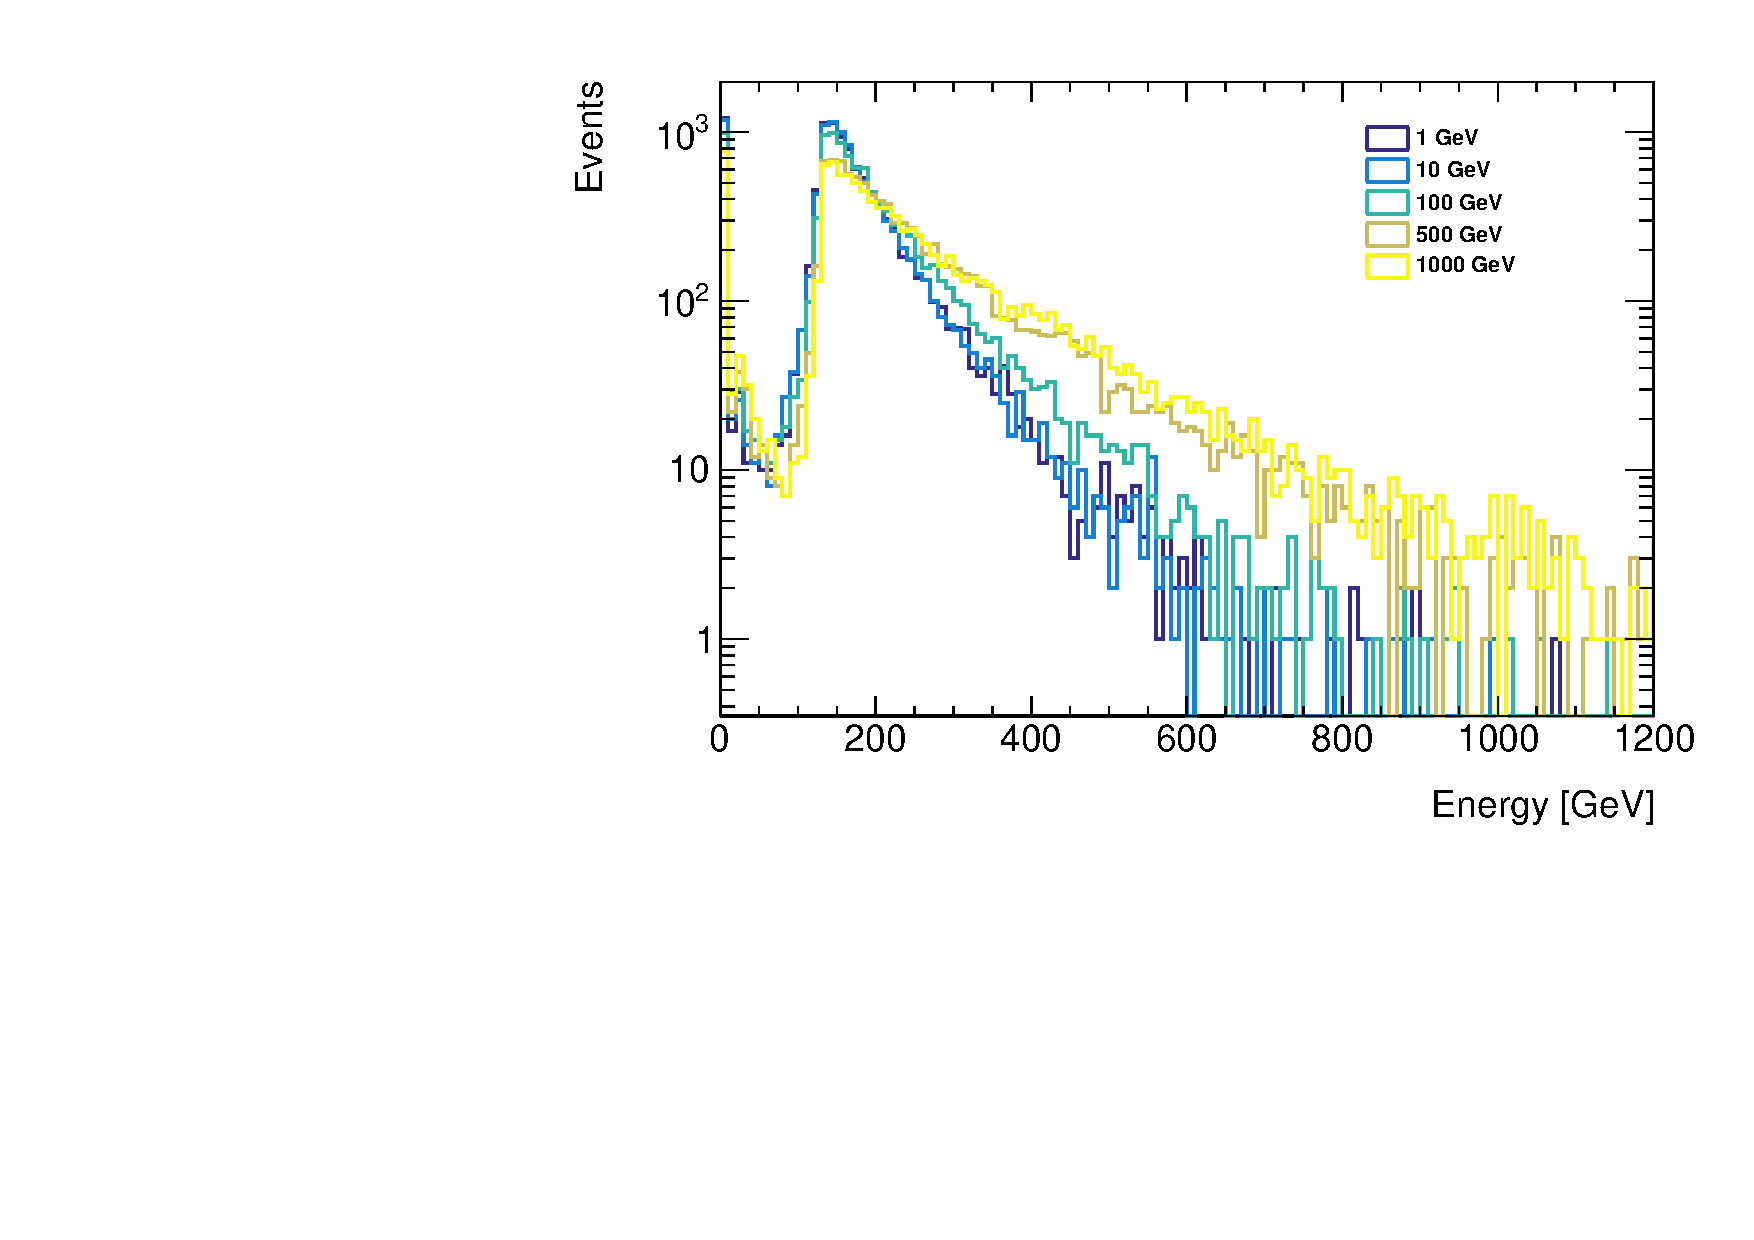
\includegraphics[width=.45\textwidth]{MCSample/canPhPtoverlap}} \quad
\subfloat[][Missing transverse momentum for different masses]
{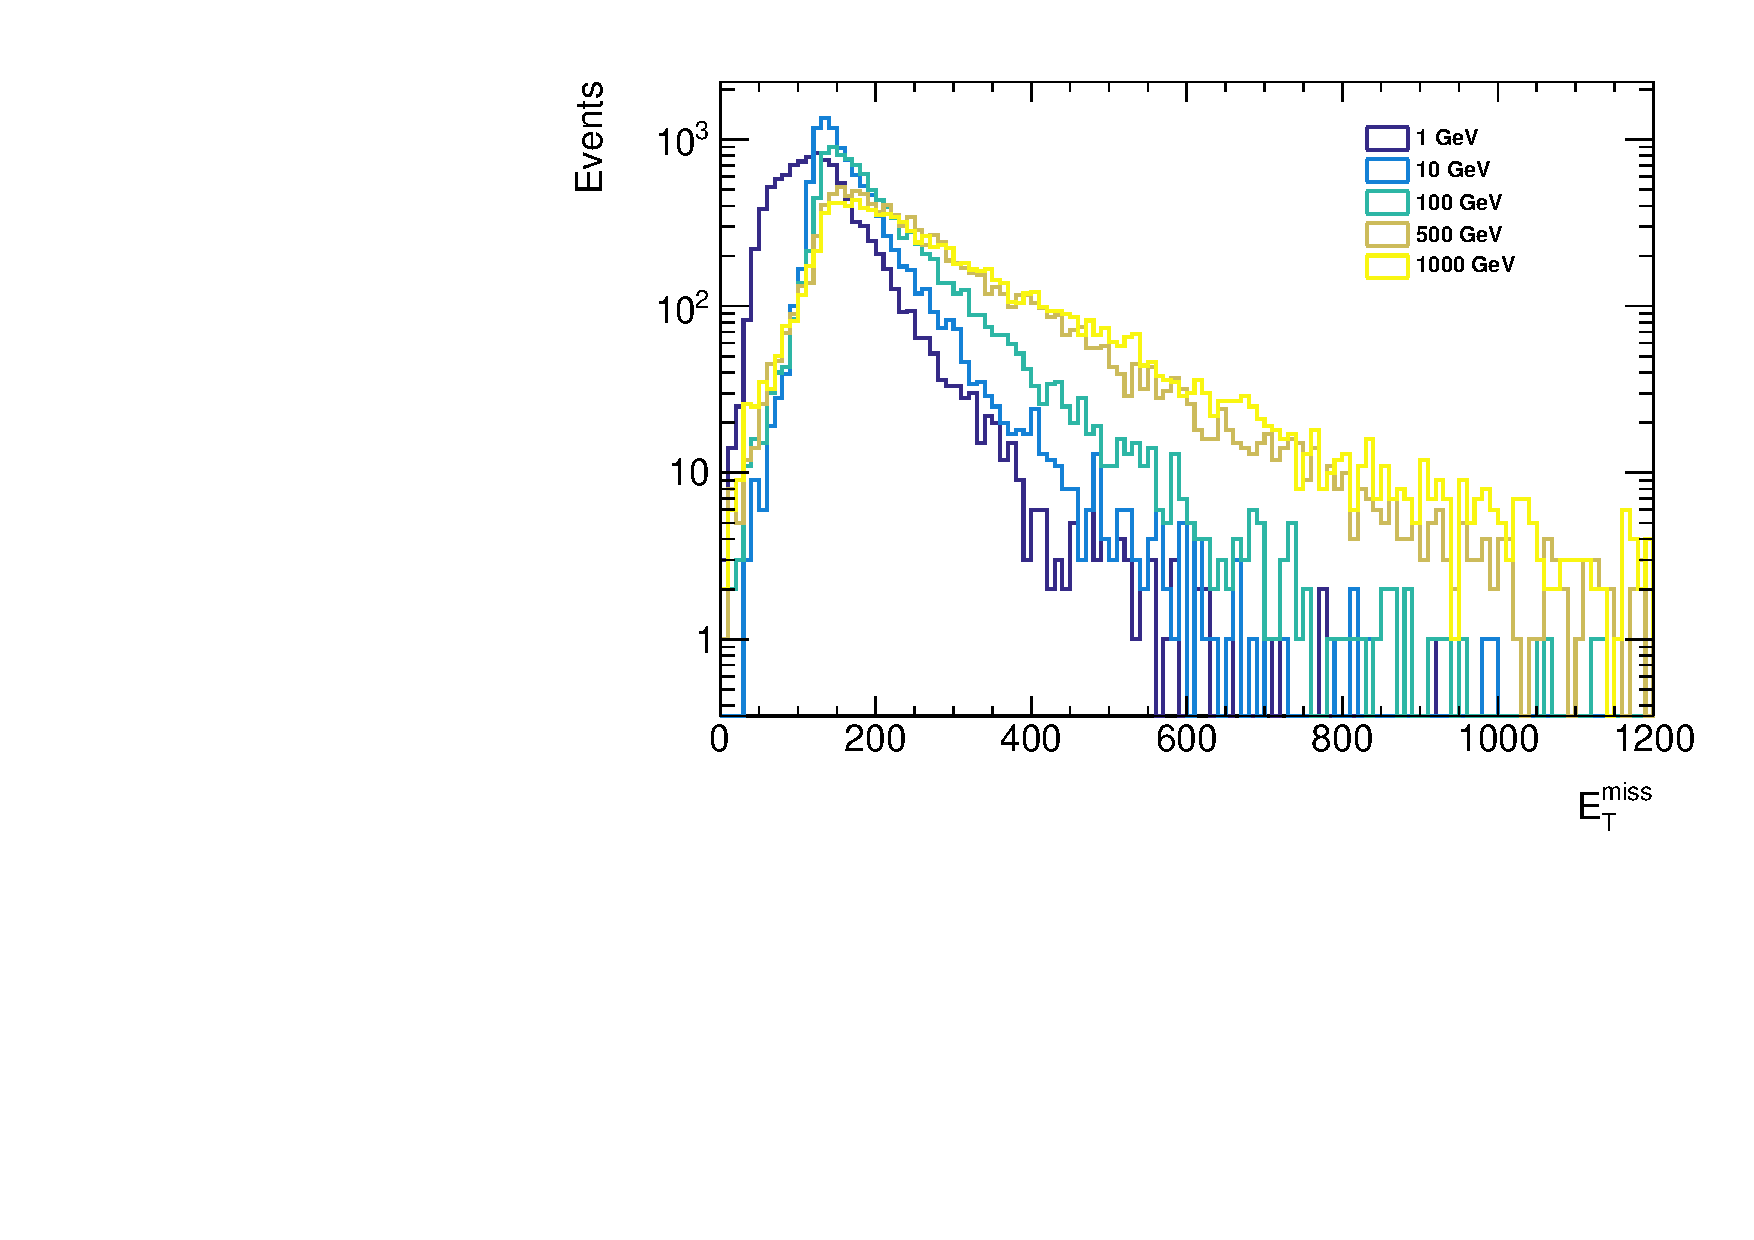
\includegraphics[width=.45\textwidth]{MCSample/canMEToverlap}} \quad
\subfloat[][Pseudorapidity of the photon for different masses]
{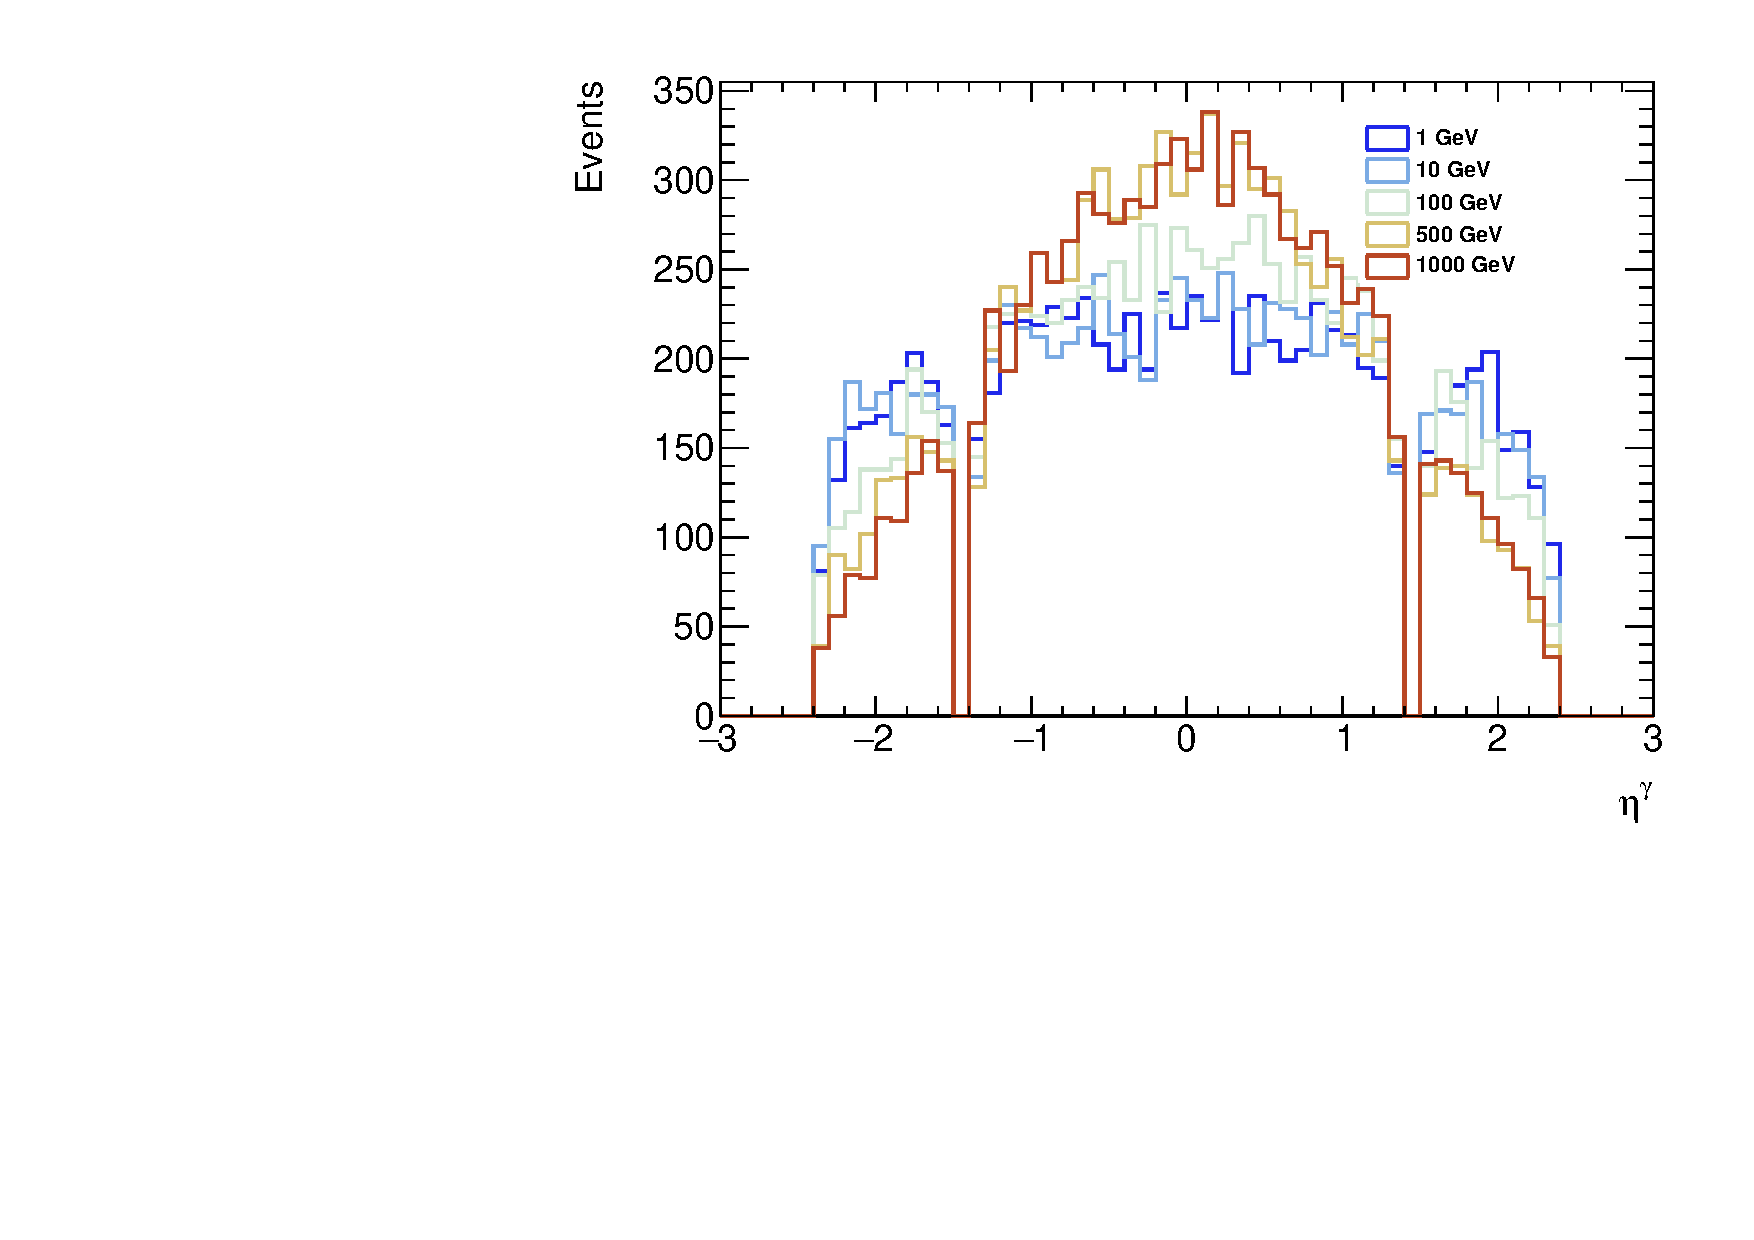
\includegraphics[width=.45\textwidth]{MCSample/canEtaoverlap}} \quad
\subfloat[][Number of jets for different masses]
{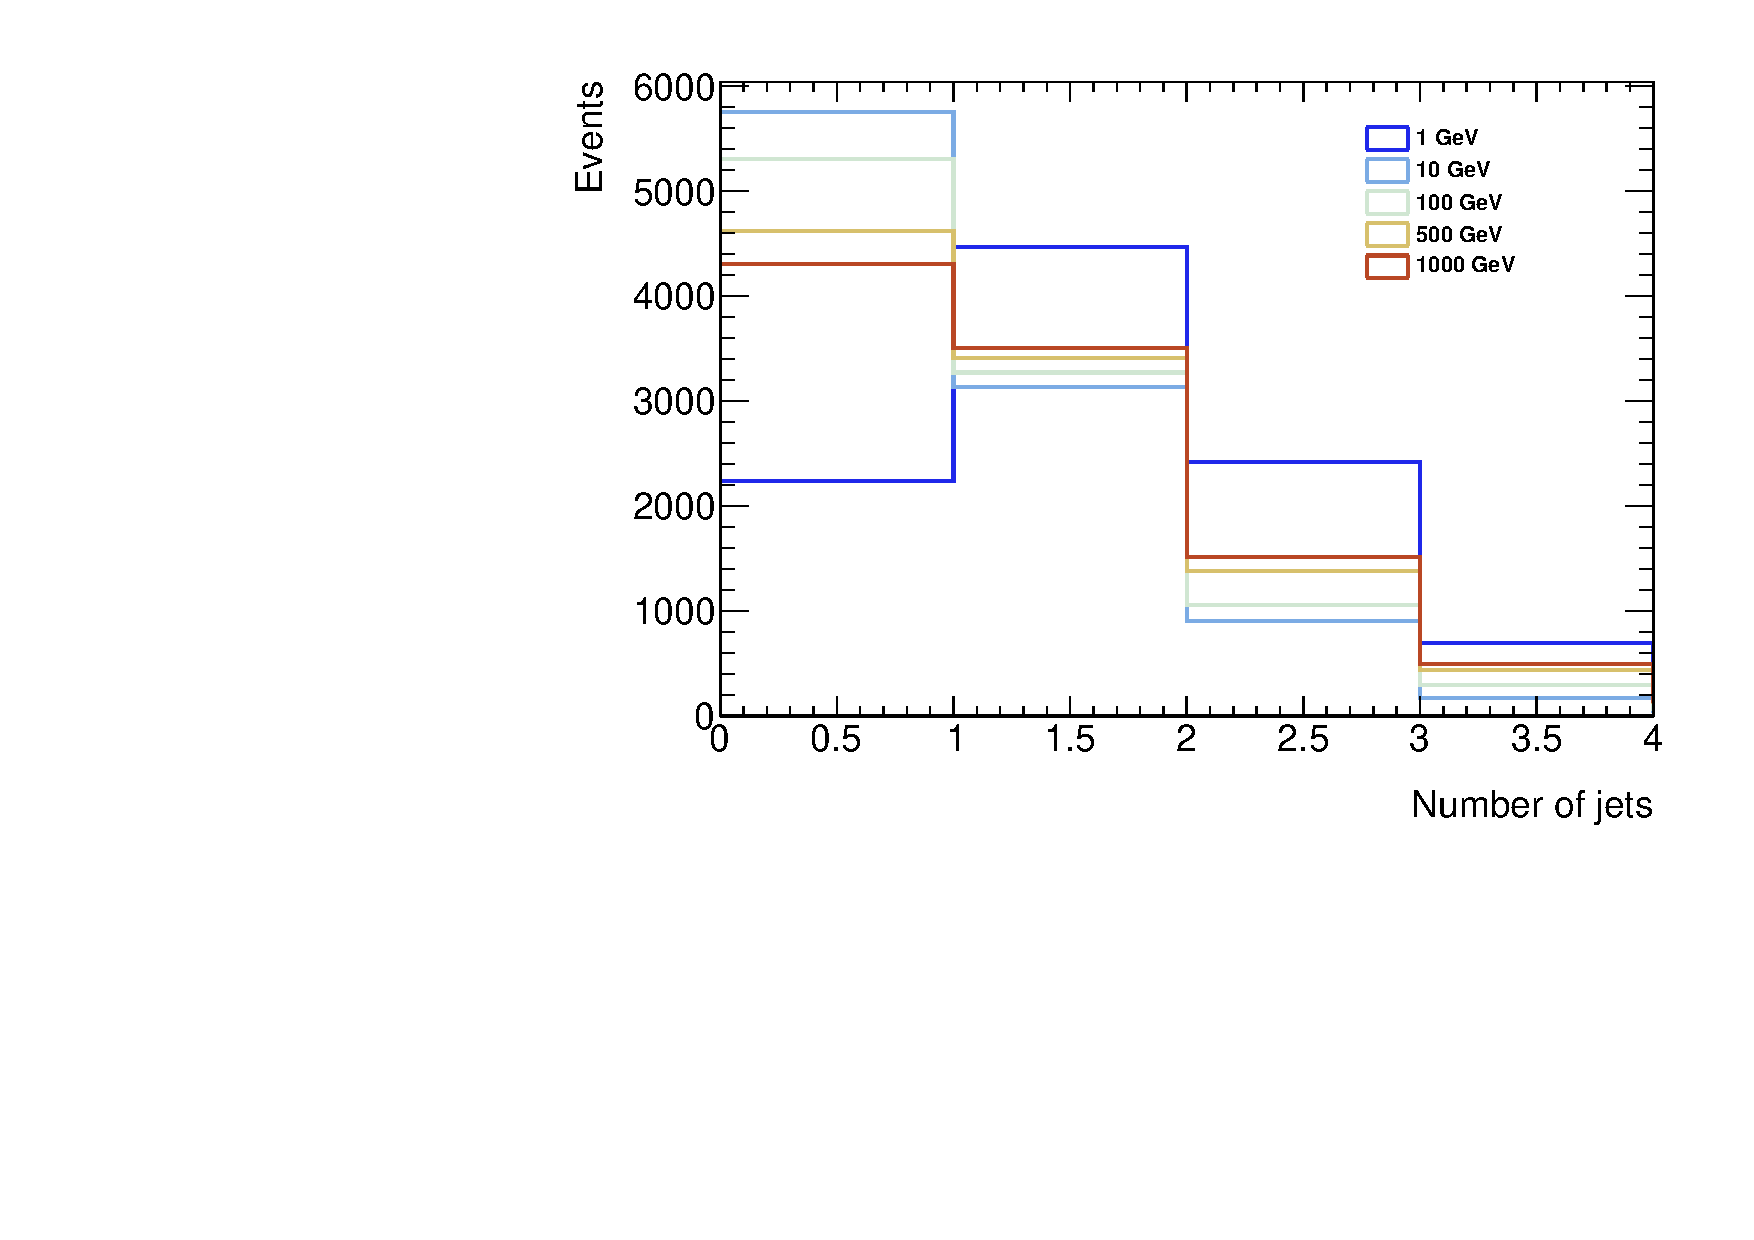
\includegraphics[width=.45\textwidth]{MCSample/canNjetsoverlap}} \quad
\caption{Validation plots for the Minimal DM model. From these plots the evolution of the main kinematics variables can be seen as a function of DM mass. These plots are generated after the pre-selection cuts given in \Sect{\ref{sec:truth}}}
\label{fig:validation}
\end{figure}

\section{Simulation}
The standard simulation of ATLAS relies on the \geant particle simulation toolkit to simulate the interaction of particles with matter. This step takes as input the EVNT file from \PYTHIA, or any of the generators such \HERWIG and \SHERPA, and it is the most time expensive stage in the full simulation. The output is stored into an HITS file. To save time the framework allows the user to skip a certain number of events at the beginning of an input file by submitting $n$ jobs with $N$ events each to a $n\times N$ event input file and merged together at the end of the process.

%First of all comes the simulation initialization which is divided in three steps. Stage one of the initialization occurs as soon as Athena is started which is set to AtlasProduction 19.2.4.9. release. Here job properties provided by the user are locked, metadata that will be stored with the hit output file are gathered and the HIT file initialized. Finally service is created to interface with \geant which is not fully initialized at this stage. In stage two detector, physics regions, range cuts are created. Each piece of the ATLAS detector is constructed in GeoModel according to the geometry chosen, which in this work is \verb!ATLAS-R2-2015-03-01-00_VALIDATION!, and translated into an equivalent \geant geometry. Next, the Monte Carlo truth strategies, which are \verb!MC12! in this context, are added to the simulation.Then the magnetic field is loaded and every user action, which allows a user to insert pieces of code in various places throughout the simulation event loop, provided from the configuration command are initialized. The physics list (see below) used for simulation is also set at this point. The third stage completes the job preparation. assigning fast simulation models and runs \geant  software.

%A physics list contains all numerical models that describe the particles' interactions in the \geant simulation. The \geant Collaboration provides several combinations of these models for every possible physical outline. We used the \verb!FTFP_BERT! phisics list which is the current \geant default. Any further information can be found in~\cite{ftfpbert}.

To speed up the full simulation process a fast simulation approach can be adopted. In this work ATLFAST-II was used, which provides large statistics to supplement full simulation studies. It is made up from two components: the Fast ATLAS Tracking Simulation (Fatras) for the inner detector and muon system simulation and the Fast Calorimeter Simulation (FastCaloSim) for the calorimeter simulation~\cite{simulation}. 

In Fatras the geometry of the detector consists in a simplified description of the full detector geometry, which maintains the same descriptive accuracy for its sensitive parts, and all other detector components are approximated as simplified layers that carry a high-granularity density providing an improvement in CPU time by a factor \num{100}. The interactions of the particles with the simplified detector layers are simulated using several methods, for instance ionization and radiative energy loss are simulated according to the Bethe-Bloch model. The photon conversion into a couple of electron and positron is performed depending on the thickness of the material crossed and hadronic interactions with the detector layer are simulated from parametric models obtained from \geant simulation results. Fatras provides also the input particle collection to give to FastCaloSim. Moreover it records energy deposition for muons in the calorimeter layers which will be used in the FastCaloSim application. The trajectories of the muons are also simulated in the muon spectrometer.

FastCaloSim uses parametrization of the longitudinal and lateral energy profile of the energy of single particle showers instead of simulating the particle interactions with the detector material. The parametrization are based on a fully-simulated, with \textsc{Geant4}, sample of 30 million events made of single photons and charged pions from an energy range between \SI{200}{\MeV} and \SI{500}{\GeV} for \AetaRange{5.0}. Electron and photon showers are approximated by the photon parametrization and hadronic showers are modeled on the charged pions.

The output from this simulation is a HITS file. The hits are records of energy deposition, with position and time, during the simulation. Most of them comes from the Inner Detector for which the majority of hits are independently stored and occupying about \SI{1360}{kB} per event while the muon system collects far fewer hits than the other subsystems and requires less disk space for the hit records (\SI{\sim3}{kB\per event}).

In order to understand anomalies and debug errors due to geometry or checking by eye overlaps and touching volumes in geometry a visualization step could also be performed. An examples of events are shown in \Fig{\ref{fig:simulation}}.

\begin{figure}[tp]
\centering
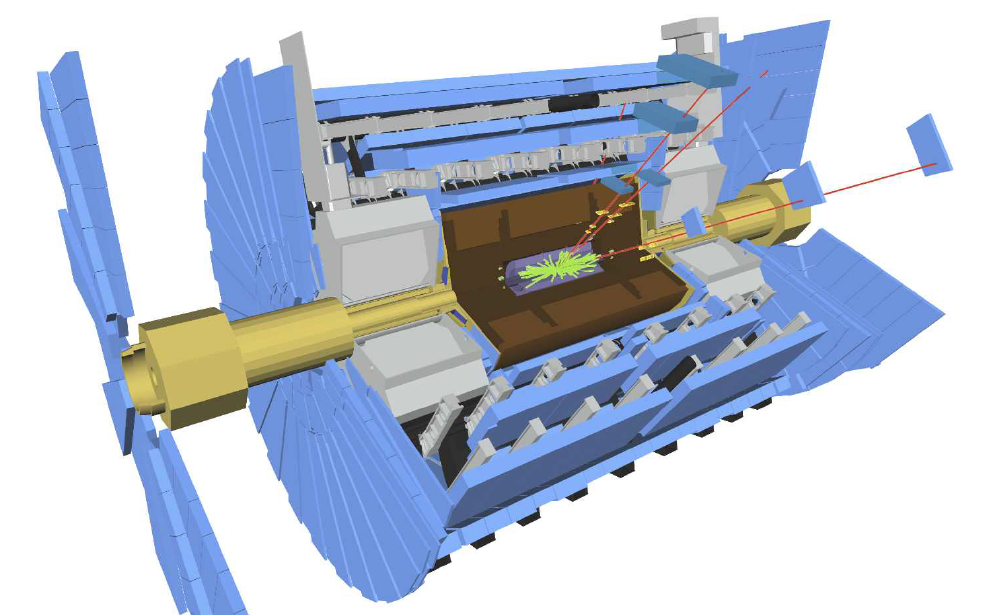
\includegraphics[width=.75\textwidth]{MCSample/simulation}
\caption{An event display made with VP1. VP1 is a viewing software made specifically for ATLAS which stands for Virtual Point 1, since ATLAS is situated at Point 1 of the LHC ring. It shows a Higgs boson decaying into four muons (shown in red). Inner detector tracks are in green, and energy deposited in the calorimeter by the muons is shown in yellow.}
\label{fig:simulation}
\end{figure}

\section{Digitization}
The ATLAS digitization software converts the hits produced by the core simulation into detector responses i.e ``digits''. In real events a digit is produced when a signal is recorded in a readout channel of the detector~\cite{simulation}.

In addition to the hard scattering digitization, \pileup and any other source of noise must be incorporated. For pile-up simulation, there are also input HITS files for minimum bias events to be overlaid, whose number for each bunch crossing is a function of the luminosity simulated. Moreover cavern background and cosmic muons could influence the simulation and they must be taken into account.
The ATLAS detector electronic produces data in byte-stream format called Raw Data Objects (RDO) whose size on disk is typically \SI{2.5}{MB\per event} and increases with larger number of \pileup events.

\section{Reconstruction}
\label{sec:recoreal}

Within this section, physics object definition and reconstruction in ATLAS are discussed, focusing on those mainly involved in this analysis. Definitions follow the recommendations from the various Combined Performance (CP) groups.

A reconstructed event in ATLAS is an ensemble of signals produced in the detector, which must be processed in order to get each particle property and identification. 

This step is identical for both real data and MC generated events and produces an output file in a Event Summary Data (ESD) and Analysis Object Data (AOD) form. 

\subsection{Photons}
\label{photons}
\subsubsection{Reconstruction}
Photons are reconstructed from clusters in the electromagnetic calorimeter measured in projective towers, even f the reconstruction uses information also from the Inner Detector. These towers are portions of the second layer of the calorimeter of $N_1 \times N_2$ cells in the $\eta-\phi$ plane. Photons and electrons (positrons) signature and energy deposits are very similar in the EM calorimeter. That's why information from ID to discriminate them are essential: a photon would not produce any track since the ID is sensitive only to charged particles. A cluster with no tracks associated is classified as a \emph{unconverted} photon since it was produced in a primary vertex it is straight revealed by the EM calorimeter. A \emph{converted} photon, instead, is produced in a primary vertex, it generates a electron-positron pair in a secondary vertex, within the ID, whose tracks can be associated to the cluster.

The reconstruction process starts from a \emph{sliding-window} algorithm which looks for the optimal deposit clusters. It starts from windows of $3\times5$ cells, or $0.025\times0.025$ in $\eta-\phi$, for unconverted photons and $3\times7$ cells ($0.175\times0.175 \, \eta\times\phi$) for converted ones, in the barrel region of the EM calorimeter, whose energy deposited is greater than \SI{2.5}{\gev}. In the end-cap, clusters of size $5\times5$ are used for all photon candidates.

%In order to identify an object as a photon or electron, tracks information is necessary. The tracking algorithm, Gaussian Sum Filter (GSF), reconstructs tracks by fitting points within the pixel detector and first layers of SCT and extrapolates informations gathered to outer layer of the ID and into the EM calorimeter. The algorithm also carefully trests the energy losses due to bremsstrahlung. Working along with the tracking algorithm, the vertexing algorithm analyses and classifies the interaction vertices and requires that a track points toward the center of the cluster whithin a $0.05\times0.05$ $\eta\times\phi$ window. Clusters with no matching tracks are classified as unconverted photons. Otherwise it is reconstructed as a converted photon or an electron.

Any noisy or sporadic noisy channel can sometimes produce a signal with transverse momentum larger than \SI{2.5}{\GeV} and give rise to a sliding window cluster~\cite{photons}. In order to identify these bad quality or fake clusters coming from instrumental problems cleaning cuts are applied on photon candidates. 

\subsubsection{Identification}
\begin{figure}[tp]
\centering
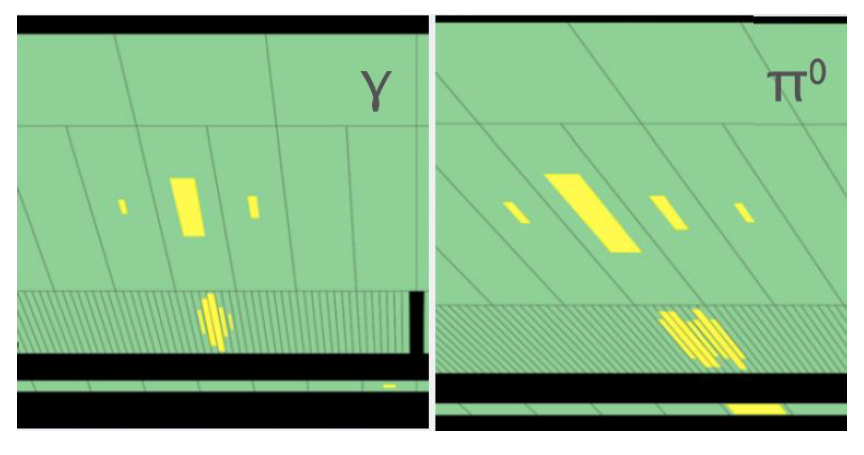
\includegraphics[width=.65\textwidth]{MCSample/pizerogamma}
\caption{Discrimination between a single photon and two collimated photons from a \pizero decay in the the ATLAS EM calorimeter. From the bottom to the top the strip, middle and back layers are visualized.}
\label{pizerogamma}
\end{figure}

Once a list of candidate photons has been made, we have to discriminate between real photons and hadronic jets containing high \pt \pizero, as shown in \Fig{\ref{pizerogamma}}. Identification is based upon the information from the strip and middle layers of the EM calorimeter.

Two working points are defined for photons: loose and tight depending on which cuts a photon passes based on shower shapes measured in strips and middle layers of the EM calorimeter together with hadronic leakage. The differences observed between data and MC in the discriminating variables are measured comparing the shower shape distributions in data and MC, parametrized as simple shifts. Instead, three working points which are loose, medium and tight, are defined for electrons. Details on photons selection criteria can be found in \cite[Sect. 4]{photons}.

Identification efficiency is computed with three different data-driven methods presented in~\cite{photons}: the matrix method, the electron extrapolation and the measurement of radiative photons from \mbox{\Zboson\rarrow\ellell$\gamma$} decays. Their efficiency comparison is given in \Fig{\ref{fig:phID}} for unconverted photons. Tight photons efficiency identification is expected to be greater than \SI{90}{\percent}.

\begin{figure}[pt]
\centering
\includegraphics[width=0.65\textwidth]{MCSample/phID}
\caption{Comparison of the data-driven measurements of the identification efficiency for unconverted photons as function of \et in the region \SIrange{10}{1500}{\gev}, for the pseudorapidity interval \AetaRange{0.6} using data collected in 2015-2016.}
\label{fig:phID}
\end{figure}

\subsubsection{Isolation}
\label{sec:phisolation}
\begin{figure}[tp]
\centering
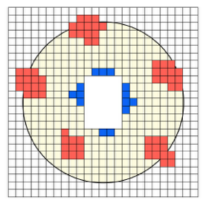
\includegraphics[width=0.4\textwidth]{MCSample/topoetcone40}
\caption{The algorithm which fills TopoEtCone40 variable in action: from the $R=0.4$ cone (yellow) a $5\times7$ rectangle is removed, energy deposited is computed among the \topo~(orange) within the cone and the \pt-leakage (blue) is subtracted.}
\label{topoetcone40}
\end{figure}

Usually the isolation of a particle is expressed in terms of the $E_\textup{T}^{\textup{iso}}$ variable, which computes the transverse energy measured in the calorimeter cells (\topo) within a cone of given radius around the candidate. A track isolation $p_\textup{T}^{\textup{iso}}$variable can be defined as well.

In the above mentioned cone, an algorithm sums up the energies of the \topo~with energy deposits above a certain threshold~\cite{photonsISO}. The contribution of the photon itself, in a $5\times7$ cells area around the cone axis, and from the underlying evens and \pileup is  subtracted and the \pt-leakage, i.e. photon energy escaped from the area previously identified, is taken into account. Then the total energy in the cone is computed and the variable storing this information in this analysis is ``TopoEtCone40'' which contains the energy evaluated in a cone of radius $R=0.4$. Therefore a photon is considered isolated if ``TopoEtCone40''remains below a certain threshold, i.e. $\text{TopoEtcone40} < 0.022\pt^\gamma + \SI{2.45}{\GeV}$ and $\text{ptcone20}/\pt^\gamma<0.05$. A visual representation of the process described is given in \Fig{\ref{topoetcone40}}.

Isolation efficiency is computed to be greater than \SI{90}{\percent} for $\et^\gamma$ greater than \SI{100}{\gev}~\cite{photonsISO}.

\subsection{Missing transverse momentum}
\label{sec:met}
\subsubsection{Reconstruction}

An intuitive definition of missing transverse momentum (\met) is the momentum inbalance in the transverse plane. A non-zero inbalance, must suggest the presence of missing energy since this plane is boost-invariant and energy must be conserved. Indeed we can state something only about transverse energy since the parton momentum in the beam direction before the collision is unknown.

The true \met is given simply by neutrinos and non interacting particles, but there are also other sources, such malfunctioning detector region or its finite coverage, that creates fake \met due to a bad or missing reconstruction of physics objects. This is particularly relevant for this analysis when we look for \emph{non}-interacting particles such DM particles.

The \met calculation used in this analysis is based on all reconstructed and calibrated physics objects. In the transverse plane the \met magnitude and the corresponding azimuthal angle are given by:
\begin{gather}
\label{eqn:met}
	\met=\sqrt{(E_x^\textup{miss})^2+(E_y^\textup{miss})^2}\\
	\phi^\textup{miss}=\arctan\big({E_y^\textup{miss}/E_x^\textup{miss}}\big)
\end{gather}

The single components $E_i^\textup{miss}$, ($i=\{x,y\}$), in equation \ref{eqn:met} is given by:
\begin{equation}
	E_i^\textup{miss}=E_i^\textup{miss,$e$}+E_i^\textup{miss,$\gamma$}+E_i^\textup{miss,$\mu$}+E_i^\textup{miss,$\tau$}+E_i^\textup{miss,jets}+E_i^\textup{miss,Soft}
\end{equation}

Each term is calculated as the negative sum of the momentum of the reconstructed objects projected onto the $x$ and $y$ direction of the transverse plane. The ``Soft'' term is calculated from energy deposits or tracks which are not matched to selected hard objects. 

There are several computation of \met, as explained in~\cite{met}. The one this analysis is based on is the ``Track Soft Term'' (TST) as recommended by ATLAS Jet/Etmiss Combined Performance groups, calculated from the tracks from the primary vertices that are not matched to selected hard objects and providing a stronger measurement against \pileup~\cite{met}.

\section{EXOT6 Derivation}
\label{sec:derivation}
During the \RunTwo ATLAS has developed a ``Derivation Framework'', by proposal by the Analysis Model Study Group (AMSG), which works on the principle that analyzers need to be able to run over their data sample frequently. For this purpose the derivation framework provides the offline software tools and structures to work on data in a very simple way~\cite{twiki:DAOD}. 

Unlike in \RunOne, when derivation was made by users, this production is now made centrally by the ATLAS production services, even if it can be run locally as in our case, avoiding difficulties in cross-team analyses due to differences in the formats and in reading the output file.

Derivations are made from the reconstructed data via four operations:
\begin{enumerate}
\item skimming: the removal of entire events;
\item thinning: when removing the whole object in an event, but keeping the rest of it;
%(for instance an electron is totally removed while other object remains),
\item slimming: information removal from objects, while keeping the rest of it; 
%(i.e. only certain object information ,such its transverse momentum. are removed but the object still remains in the event),
\item augmentation: adding informations not found in the input data.
\end{enumerate}

Therefore the derivation framework selects only the relevant data for a specific analysis, from all ATLAS data collected. This functioning is well explained in the sketch shown in \Fig{\ref{fig:derivation}}.

For this analysis a specific derivation called ``EXOT6'' has been implemented and the following skimming selection was applied:
\begin{itemize}
\item Events must pass one out of several trigger request, including the \verb!HLT_g140_loose! which this analysis is based on;
\item Events must have one loose
%\footnote{see \Sect{\ref{photons}}} 
photon with $\pt\ge\SI{80}{\gev}$ or one loose electron with \mbox{$\pt\ge\SI{100}{\gev}$}.
\end{itemize}

As final step a ROOT::NTUPLE file was produced in which events are selected following the recommendation by the Combined Performance groups. The analysis code is based on SUSYTools-00-08-20 based on AnalysisBase 2.4.28. Details on object definition and kinematic cuts performed in the SUSYTools code are given in~\cite{twiki:SUSYTools}.


\begin{figure}[tb]
\centering
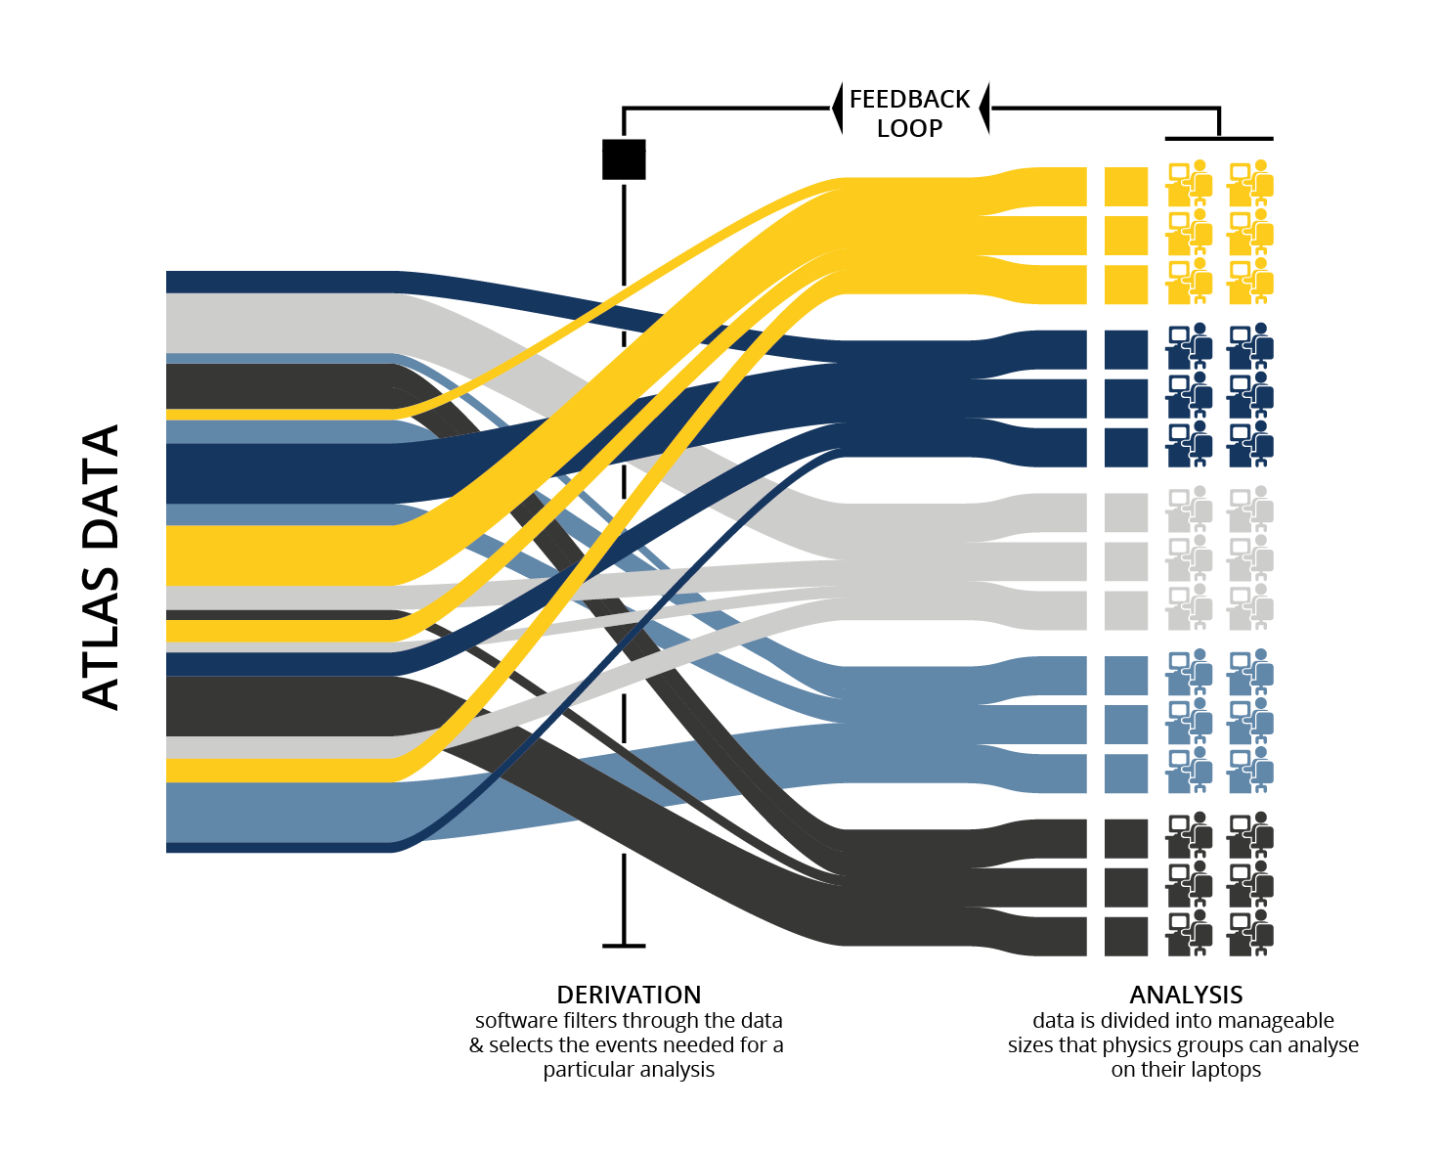
\includegraphics[width=.48\textwidth]{MCSample/Derivation}
\caption{Sketch of how the derivation code works for ATLAS data. Each single event from the whole amount of dara contains different characteristics that the derivation code depending on the analysis performed.}
\label{fig:derivation}
\end{figure}















